\chapter{Discussion}
Please tell more about conclusion and how to the next work of this study.

\section{Andi Muhammad Aslam/1164064}
\subsection{Teori}
\begin{enumerate}
\item Jelaskan kenapa file teks harus di lakukan tokenizer.
\subitem Tahap Tokenizing adalah tahap pemotongan string input berdasarkan tiap kata yang menyusunnya. Tokenisasi secara garis besar memecah sekumpulan karakter dalam suatu teks ke dalam satuan kata, bagaimana membedakan karakter-karakter tertentu yang dapat diperlakukan sebagai pemisah kata atau bukan. Sebagai contoh karakter whitespace, seperti enter, tabulasi, spasi dianggap sebagai pemisah kata. Namun untuk karakter petik tunggal (‘), titik (.), semikolon (;), titk dua (:) atau lainnya, dapat memiliki peran yang cukup banyak sebagai pemisah kata.
\begin{figure}[!htbp]
	\centerline{\includegraphics[width=1\textwidth]{figures/andi/7-1.PNG}}
	\caption{Tokenizer}
	\label{Teori}
\end{figure}

\item Jelaskan konsep dasar K Fold Cross Validation pada dataset komentar Youtube pada kode listing 7.1.dilengkapi dengan ilustrasi atau gambar.
\subitem Starfiedkfold yaitu mengembalikan lipatan data bertingkat. Lipatan dibuat dengan mempertahankan presentase sampel setiap kelas dari dataset youtube. dari contoh sampel dalam ilustrasi mempresentasikan sampel dataset menjadi 5 bagian di setiap kelasnya.

\begin{lstlisting}[caption=K Fold Cross Validation,label={lst:7.0}]
kfold = StratifiedKFold(n_splits=5)
splits = kfold.split(d, d['CLASS'])
\end{lstlisting}

\item Berikut ilustrasi pada K Fold Cross Validation :
\begin{figure}[ht]
\centering
\includegraphics[scale=0.5]{figures/andi/7-2.PNG}
\caption{ KFold Cross validation}
\label{Teori}
\end{figure}

\item Jelaskan apa maksudnya kode program for train, test in splits. dilengkapi denganilustrasi atau gambar.
\subitem Maksudnya For Train, test in split untuk menguji dataset yang sudah di split sebelumnya agar tidak terjadi penumpukkan, yaitu dengan cepat dapat mengelompokkan validasi input data dan dapat di ShuffleSplit dan aplikasi untuk memasukkan data ke dalam satu panggilan tunggal agar dapat memisahkan data secara opsional dan subsampling.

\item Berikut ilustrasi pada for train, test in splits :
\begin{figure}[ht]
\centering
\includegraphics[scale=0.5]{figures/andi/7-3.PNG}
\caption{Ilustrasi for train, test in splits}
\label{Teori}
\end{figure}

\item Jelaskan apa maksudnya kode program train content = d[’CONTENT’].iloc[train idx] dan test content = d[’CONTENT’].iloc[test idx]. dilengkapi dengan ilustrasi atau gambar.
\subitem Maksudnya untuk mengambil data pada Index CONTENT yang merupakan bagian dari train\_idx dan test\_idx. 
Ilustrasi, apabila data diubah menjadi train content dan test content maka kita dapat memilih content apa yang ingin di tampilkan pada kolom.

\item Jelaskan apa maksud dari fungsi tokenizer = Tokenizer(num words=2000) dan tokenizer.fit on texts(train content), dilengkapi dengan ilustrasi atau gambar.
\subitem Dimana Tokenizer yang akan melakukan vektorisasi pada kata yang dimana jumlah kata yang ingin diubah kedalam bentuk token adalah 2000 kata. Untuk tokenizer.fit on texts(train content) maksudnya yaitu untuk melakukan fit tokenizer hanya untuk data train saja, tidak berlaku pada data test nya untuk kolom CONTENT. Ilustrasi, " bayi itu sedang tertidur lelap" maksudnya ini akan membuat kamus s.t word\_index ["tidur"] = 0; word\_index ["bayi"] = 1; itu merupakan kata  kamus indeks sehingga setiap kata mendapatkan nilai integer yang unik.
\begin{figure}[!htbp]
	\centerline{\includegraphics[width=1\textwidth]{figures/andi/7-5.PNG}}
	\caption{Fungsi Tokenizer}
	\label{Teori}
\end{figure}

\item Jelaskan apa maksud dari fungsi d train inputs = tokenizer.texts to matrix(train content, mode=’tfidf’) dan d test inputs  tokenizer.texts to matrix(test content, mode=’tfidf’), dilengkapi dengan ilustrasi kode dan atau gambar.
\subitem fungsi tersebut yang akan membagi matrix TF IDF dengan amax yaitu mengembalikan nilai max array atau nilai max sepanjang sumbu. yang hasilnya akan dimasukkan kedalam variable (train input) untuk daata train dan (test input) untuk data test dengan nominal tanpa adanya bilangan negatif dan koma.
\begin{figure}[!htbp]
	\centerline{\includegraphics[width=1\textwidth]{figures/andi/7-6.JPG}}
	\caption{Matrix TF IDF}
	\label{Teori}
\end{figure}

\item Jelaskan apa maksud dari fungsi d train inputs = d train inputs/np.amax(np.absolute(d train dan d test inputs = d test inputs/np.amax(np.absolute(d test inputs)), dilengkapi dengan ilustrasi atau gambar.
\subitem Fungsi tersebut akan membagi matrix tfidf tadi dengan amax yaitu mengembalikan maksimum array atau maksimum sepanjang sumbu. Yang hasilnya akan dimasukan kedalam variabel d\_train\_inputs untuk data train dan d\_test\_inputs untuk data test dengan nominal absolut atau tanpa ada bilangan negatif dan koma.
\begin{figure}[!htbp]
	\centerline{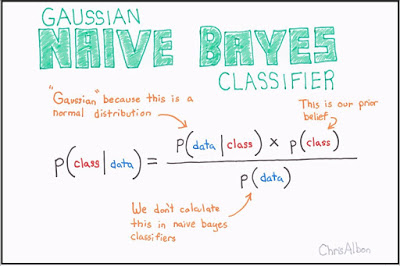
\includegraphics[width=1\textwidth]{figures/andi/7-7.PNG}}
	\caption{Matrix TFID}
	\label{Teori}
\end{figure}

\item Jelaskan apa maksud fungsi dari d train outputs = np utils.to categorical(d['CLASS'].iloc[train dan d test outputs = np utils.to categorical(d['CLASS'].iloc[test idx]) dalam kode program.
\subitem maksud dari fungsi tersebut yaitu untuk merubah nilai vektor yang ada pada atribut class menjadi bentuk matrix dengan pengurutan berdasarkan data index training dan testing.
\begin{figure}[!htbp]
	\centerline{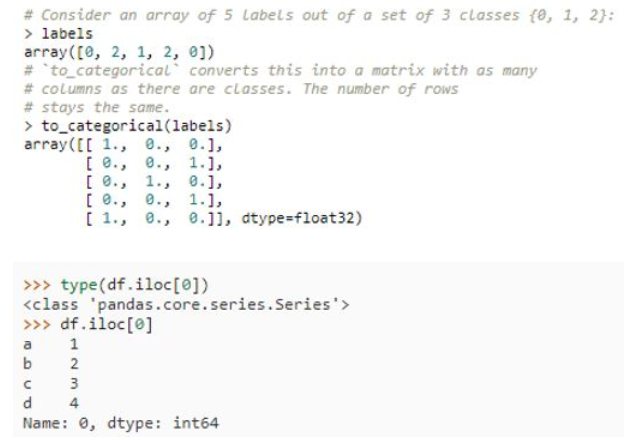
\includegraphics[width=1\textwidth]{figures/andi/7-8.PNG}}
	\caption{Matrix Training dan Testing}
	\label{Teori}
\end{figure}

\item Jelaskan apa maksud dari fungsi di listing.
 \lstinputlisting{src/1164064/chapter7-9.py}
\item Dari fungsi pada kode program tersebut ditujukan untuk melakukan pemodelan dengan sequential, membandingkan setiap satu larik elemen dengan cara satu persatu secara beruntun. Dimana terdapat 512 neuron inputan dengan input shape 2000 vektor. Lalu model dilakukan aktivasi dengan fungsi 'relu'. Kemudian dilakukan pemotongan bobot supaya tidak overfitting sebesar 50 persen dari neuron inputan 512. Lalu pada layer output terdapat 2 neuron outputan yaitu nol(1,0) atau nol satu(0,1). Kemudian outputan tersebut diaktivasi menggunakan fungsi softmax.
\par 


\item Jelaskan apa maksud dari fungsi di listing.
\lstinputlisting{src/1164064/chapter7-10.py}
\begin{itemize}
\item  Dari fungsi pada kode program tersebut model yang telah dibuat selanjutnya dicompile dengan menggunakan algoritma optimisasi dengan fungsi-fungsi loss, fungsi opttimaizer dan fungsi metrik. Dimana nama masing-masing fungsi tersebut adalah categorical\_crossentropy, adamax dan accuracy.
\par 
\end{itemize}
\par
\par

\item Jelaskan apa itu Deep Learning.
\subitem Deep Learning adalah salah satu jenis algoritma jaringan saraf tiruan yang menggunakan metadata sebagai input dan mengolahnya menggunakan sejumlah lapisan tersembunyi (hidden layer) transformasi non linier dari data masukan untuk menghitung nilai output. Algortima pada Deep Learning memiliki fitur yang unik yaitu sebuah fitur yang mampu mengekstraksi secara otomatis.

\item Jelaskan apa itu Deep Neural dan bedanya dengan Deep Learning.
\subitem Deep Neural Network atau DNN merupakan algoritma yang berbasis neural network yang digunakan untuk mengambil keputusan.

\item Yang membedakan Deep Learning dengan  Deep Neural Network (DNN) 
\subitem DNN merupakan algoritma yang digunakan pada Deep Learning, sedangkan Deep Learning merupakan model yang menggunakan algoritma DNN.


\item Jelaskan dengan ilustrasi gambar buatan sendiri(langkah per langkah) bagaimana perhitungan algoritma konvolusi dengan ukuran stride (NPM mod3+1) x (NPM mod3+1) yang terdapat max pooling.
\subitem Konvolusi pada gambar dilakukan dalam image processing untuk menerapkan operator yang memiliki nilai output dari piksel gambar yang berasal dari kombinasi linear nilai input piksel, semakin nilai piksel tersebut maka kualitas gambar bisa semakin bagus.
\begin{figure}[!htbp]
	\centerline{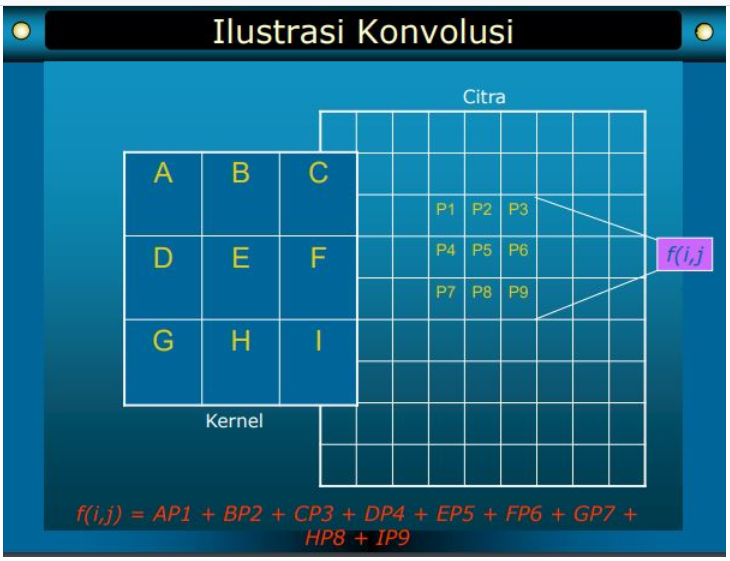
\includegraphics[width=1\textwidth]{figures/andi/7-131.PNG}}
	\caption{Konvolusi}
	\label{Teori}
\end{figure}

\begin{figure}[!htbp]
	\centerline{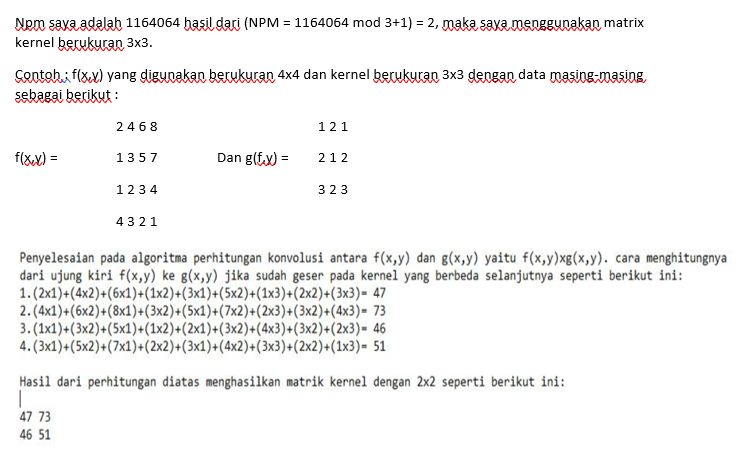
\includegraphics[width=1\textwidth]{figures/andi/7-132.PNG}}
	\caption{Algoritma Perhitungan Konvolusi}
	\label{Teori}
\end{figure}

\end{enumerate}

\subsection{Praktek Program}
\begin{enumerate}
\item Jelaskan kode program pada blok \# In[1]
\par Berikut adalah kode program yang digunakan :
\lstinputlisting[firstline=2, lastline=4, caption=Kode Program 1, label={1}]{src/1164064/MathSymbols.py}
\par Dari kode listing pada kode program 1, dapat dijelaskan seperti berikut :
\begin{itemize}
\item Baris 1	: Melakukan pengimportan file csv
\item Baris 2	: Melakukan pemanggilan atau memasukkan module image sebagai pil\_image dari library PIL
\item Baris 3	: Melakukan pengimportan fungsi keras.processing.image 
\end{itemize}
\begin{figure}[!htbp]
	\centerline{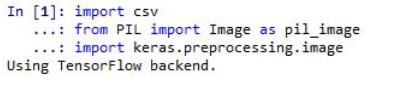
\includegraphics[width=1\textwidth]{figures/andi/p1.PNG}}
	\caption{In[1]}
\end{figure}
\item Jelaskan kode program pada blok \# In[2]
\par Berikut adalah kode program yang digunakan :
\lstinputlisting[firstline=8, lastline=21, caption=Kode Program 2, label={2}]{src/1164064/MathSymbols.py}
\par Dari kode listing pada kode program 2, dapat dijelaskan seperti berikut :
\begin{itemize}
\item Baris 1	: Membuat variabel imgs tanpa ada parameter di dalamnya
\item Baris 2	: Membuat variabel classes tanpa ada parameter didalamnya
\item Baris 3	: Membuka file csv dari HASYv2/hasy-data-labels.csv sebagai csvfile
\item Baris 4	: Membuat variabel csvreader yang difungsikan untuk membaca dari file csv yang dimasukkan
\item Baris 5	: Membuat variabel i dengan parameter 0 atau nilai 0
\item Baris 6	: Digunakan untuk melakukan eksekusi baris dari pembacaan csv 
\item Baris 7	: Mengaplikasikan atau menggunakan perintah "if" dengan variabel i lebih besar dari 0, yang selanjutnya akan dilanjutkan ke perintah berikutnya
\item Baris 8	: Membuat variabel img yang berfungsi untuk mengubah image atau gambar menjadi bentuk array (bilangan) dari file HASYv2 yang dibuka dengan row berparameter 0.
\item Baris 9	: Membuat variabel img dengan nilai bukan sama dengan 255.0
\item Baris 10 : Mendefinisikan fungsi imgs.append yang digunakan untuk melakukan proses penggabungan data dengan file lain atau dataset lain yang telah ditentukan dengan 3 parameter yaitu row[0], row[2] dan variabel img.
\item Baris 11 : Mendefinisikan fungsi append dari variabel classes dengan menggunakan parameter row[2].
\item Baris 12 : Mengartikan i=i+1 yang dimana nilai sari variabel i akan ditambah 1 sehingga akan bernilai 1.
\end{itemize}
\par Sehingga dari kode program tersebut bila dijalankan, maka menghasilkan seperti pada gambar 
\begin{figure}[!htbp]
	\centerline{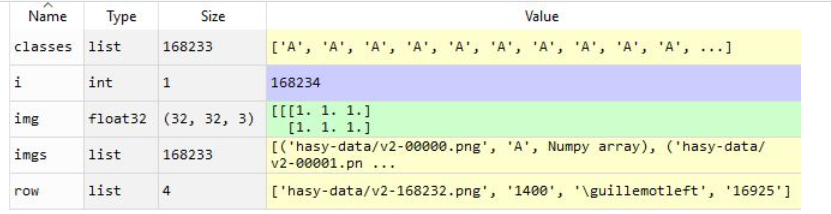
\includegraphics[width=1\textwidth]{figures/andi/p2.PNG}}
	\caption{In[2]}
	
\end{figure}
\item Jelaskan kode program pada blok \# In[3]
\par Berikut adalah kode program yang digunakan :
\lstinputlisting[firstline=25, lastline=29, caption=Kode Program 3, label={3}]{src/1164064/MathSymbols.py}
\par Dari kode listing pada kode program 3, dapat dijelaskan seperti berikut :
\begin{itemize}
\item Baris 1	: Memanggil dan menggunakan module random
\item Baris 2	: Melakukan pengocokan menggunakan module random pada parameter variabel imgs
\item Baris 3	: Membagi index data kedalam bentuk integer dengan mengalikan 0,8 dan len yang berfungsi mengembalikan jumlah item dalam datanya dari variabel imgs
\item Baris 4	: Membuat variabel train yang digunakan untuk mengeksekusi imgs serta pemecahan index awal pada data untuk digunakan sebagai data training
\item Baris 5	: Membuat variabel test yang digunakan untuk mengeksekusi imgs serta pemecahan index akhir pada data untuk digunakan sebagai data testing
\end{itemize}
\par Sehingga dari kode program tersebut bila dijalankan, maka menghasilkan seperti pada gambar
\begin{figure}[!htbp]
	\centerline{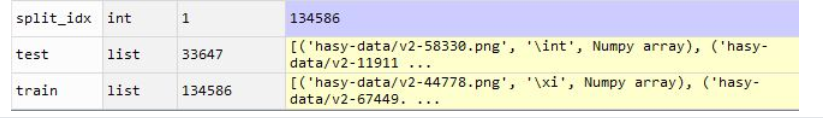
\includegraphics[width=1\textwidth]{figures/andi/p3.PNG}}
	\caption{In[3]}
	
\end{figure}
\item Jelaskan kode program pada blok \# In[4]
\par Berikut adalah kode program yang digunakan :
\lstinputlisting[firstline=33, lastline=39, caption=Kode Program 4, label={4}]{src/1164064/MathSymbols.py}
\par Dari kode listing pada kode program 4, dapat dijelaskan seperti berikut :
\begin{itemize}
\item Baris 1	: Melakukan import library numpy sebagai np
\item Baris 2	: Membuat variabel train\_input untuk mengubah inputan menjadi array menggunakan fungsi np.asarray dan  fungsi list untuk mengkoleksi data yang dipilih serta data dapat diubah. Dan didalamnya melakukan penerapan fungsi map yang berfungsi untuk mengembalikan iterator dari data yang digunakan dan fungsi lamda pada row berparameter [2] difungsikan untuk membuat objek menjadi lebih kecil sehingga mudah dieksekusi dari variabel train.
\item Baris 3	: Membuat variabel test\_input untuk mengubah inputan menjadi array menggunakan fungsi np.asarray dan  fungsi list untuk mengkoleksi data yang dipilih serta data dapat diubah. Dan didalamnya melakukan penerapan fungsi map yang berfungsi untuk mengembalikan iterator dari data yang digunakan dan fungsi lamda pada row berparameter [2] difungsikan untuk membuat objek menjadi lebih kecil sehingga mudah dieksekusi dari variabel test.
\item Baris 4	: Membuat variabel train\_input untuk mengubah inputan menjadi array menggunakan fungsi np.asarray dan  fungsi list untuk mengkoleksi data yang dipilih serta data dapat diubah. Dan didalamnya melakukan penerapan fungsi map yang berfungsi untuk mengembalikan iterator dari data yang digunakan dan fungsi lamda pada row berparameter [1] difungsikan untuk membuat objek menjadi lebih kecil sehingga mudah dieksekusi dari variabel train.
\item Baris 5	: Membuat variabel test\_input untuk mengubah inputan menjadi array menggunakan fungsi np.asarray dan  fungsi list untuk mengkoleksi data yang dipilih serta data dapat diubah. Dan didalamnya melakukan penerapan fungsi map yang berfungsi untuk mengembalikan iterator dari data yang digunakan dan fungsi lamda pada row berparameter [1] difungsikan untuk membuat objek menjadi lebih kecil sehingga mudah dieksekusi dari variabel test.
\end{itemize}
\par Sehingga dari kode program tersebut bila dijalankan, maka menghasilkan seperti pada gambar 
\begin{figure}[!htbp]
	\centerline{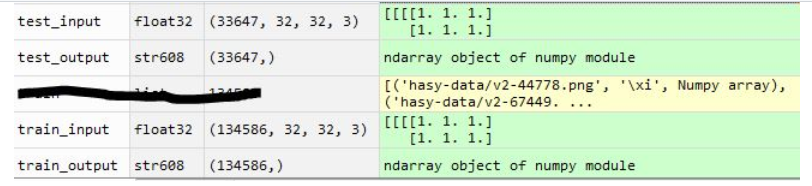
\includegraphics[width=1\textwidth]{figures/andi/p4.PNG}}
	\caption{In[4]}
	
\end{figure}
\item Jelaskan kode program pada blok \# In[5]
\par Berikut adalah kode program yang digunakan :
\lstinputlisting[firstline=42, lastline=43, caption=Kode Program 5, label={5}]{src/1164064/MathSymbols.py}
\par Dari kode listing pada kode program 5, dapat dijelaskan seperti berikut :
\begin{itemize}
\item Baris 1	: Menggunakan fungsi LabelEncoder dari sklearn.processing yang berfungsi untuk menormalkan label dimana label encoder hanya didefinisikan dengan nilai antara 0 dan -1.
\item Baris 2	: Menggunakan fungsi OneHotEncoder dari sklearn.processing yang berfungsi untuk mendefinisikan fitur input yang dimana mengambil nilai dalam kisaran [0, nilai maksimal].
\end{itemize}
\par Sehingga dari kode program tersebut bila dijalankan, maka menghasilkan seperti pada gambar 
\begin{figure}[!htbp]
	\centerline{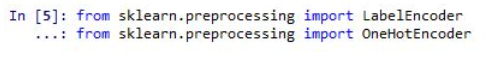
\includegraphics[width=1\textwidth]{figures/andi/p5.PNG}}
	\caption{In[5]}
	
\end{figure}
\item Jelaskan kode program pada blok \# In[6]
\par Berikut adalah kode program yang digunakan :
\lstinputlisting[firstline=48, lastline=49, caption=Kode Program 6, label={6}]{src/1164064/MathSymbols.py}
\par Dari kode listing pada kode program 6, dapat dijelaskan seperti berikut :
\begin{itemize}
\item Baris 1	: Membuat variabel label\_encoder dengan penerapan modul / fungsi LabelEncoder tanpa parameter
\item Baris 2	: Membuat variabel integer\_encoded dengan penerapan fungsi label\_encoder.fit\_transform yang berfungsi untuk melakukan ekstrasi fitur object dari variabel classes yang akan mengembalikan beberapa data yang diubah kembali.
\end{itemize}
\par Sehingga dari kode program tersebut bila dijalankan, maka menghasilkan seperti pada gambar 
\begin{figure}[!htbp]
	\centerline{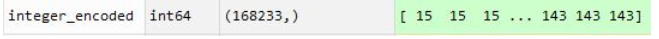
\includegraphics[width=1\textwidth]{figures/andi/p6.PNG}}
	\caption{In[6]}
	
\end{figure}
\item Jelaskan kode program pada blok \# In[7]
\par Berikut adalah kode program yang digunakan :
\lstinputlisting[firstline=52, lastline=54, caption=Kode Program 7, label={7}]{src/1164064/MathSymbols.py}
\par Dari kode listing pada kode program 7, dapat dijelaskan seperti berikut :
\begin{itemize}
\item Variabel onehot\_encoder akan memanggil fungsi OneHotEncoder dimana tidak berisikan matriks sparse.
\item Pada variabel integer\_encoded akan diubah bentuknya dimana setiap nilai integer akan direpresentasikan sebagai vektor binari dengan nilai 0 kecuali index dari integer tersebut ditandai dengan 1.
\item Melakukan fit untuk one hot encoder kedalam integer\_encoder.
\end{itemize}
\par Sehingga dari kode program tersebut bila dijalankan, maka menghasilkan seperti pada gambar 
\begin{figure}[!htbp]
	\centerline{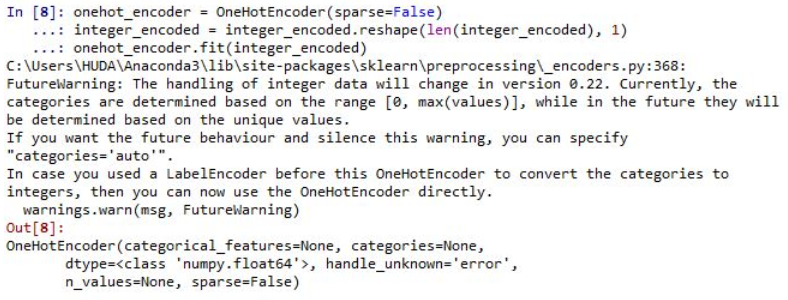
\includegraphics[width=1\textwidth]{figures/andi/p7.PNG}}
	\caption{In[7]}
	
\end{figure}
\item Jelaskan kode program pada blok \# In[8]
\par Berikut adalah kode program yang digunakan :
\lstinputlisting[firstline=57, lastline=63, caption=Kode Program 8, label={8}]{src/1164064/MathSymbols.py}
\par Dari kode listing pada kode program 8, dapat dijelaskan seperti berikut :
\begin{itemize}
\item Variabel train\_output\_int  akan mengubah data dari train\_output menjadi LabeEncoder
\item Dimana pada train\_output setelah diubah labelnya menjadi integer dilakukan one hot encoding diambil dari train\_output\_int dan menggunakan .reshape untuk memberikan bentuk baru ke array tanpa mengubah datanya dengan keterangan jika index dari integer tersebut ditandai dengan 1 dan sisanya yang bukan nol.
\item Variabel test\_output\_int  akan mengubah data dari test\_output menjadi LabeEncoder
\item Dimana pada train\_output setelah diubah labelnya menjadi integer dilakukan one hot encoding diambil dari test\_output\_int dan menggunakan .reshape untuk memberikan bentuk baru ke array tanpa mengubah datanya dengan keterangan jika index dari integer tersebut ditandai dengan 1 dan sisanya yang bukan nol.
\item Variabel num\_classes akan menampilakn jumlah data dari classes yang telah dilakukan label encoder
\item Menampilkan tulisan "Number of classes : \%d dmana mengembalikan nilai integer dari num\_classes.
\end{itemize}
\par Sehingga dari kode program tersebut bila dijalankan, maka menghasilkan seperti pada gambar 
\begin{figure}[!htbp]
	\centerline{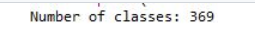
\includegraphics[width=1\textwidth]{figures/andi/p8.PNG}}
	\caption{In[8]}
	
\end{figure}
\item Jelaskan kode program pada blok \# In[9]
\par Berikut adalah kode program yang digunakan :
\lstinputlisting[firstline=67, lastline=69, caption=Kode Program 9, label={9}]{src/1164064/MathSymbols.py}
\par Dari kode listing pada kode program 9, dapat dijelaskan seperti berikut :
\begin{itemize}
\item Impor Sequential dari model pada librari Keras.
\item Impor Dense, Dropout, Flatten dari modul Layers pada librari Keras.
\item Impor Conv2D, MaxPooling2D dari modul Layers pada librari Keras.
\end{itemize}
\par Sehingga dari kode program tersebut bila dijalankan, maka menghasilkan seperti pada gambar 
\begin{figure}[!htbp]
	\centerline{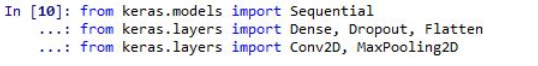
\includegraphics[width=1\textwidth]{figures/andi/p9.PNG}}
	\caption{In[9]}
	
\end{figure}
\item Jelaskan kode program pada blok \# In[10]
\par Berikut adalah kode program yang digunakan :
\lstinputlisting[firstline=71, lastline=85, caption=Kode Program 10, label={10}]{src/1164064/MathSymbols.py}
\par Dari kode listing pada kode program 10, dapat dijelaskan seperti berikut :
\begin{itemize}
\item Melakukan pemodelan Sequential.
\item Menambahkan Konvolusi 2D dengan 32 filter konvolusi masing-masing berukuran 3x3 dengan algoritam activation relu dengan data dari train\_input mulai dari baris nol.
\item Menambahkan Max Pooling dengan matriks 2x2.
\item Dilakukan lagi penambahkan Konvolusi 2D dengan 32 filter konvolusi masing-masing berukuran 3x3 dengan algoritam activation relu.
\item Menambahkan lagi Max Pooling dengan matriks 2x2.
\item Mendefinisikan inputan dengan 1024 neuron dan menggunakan algoritma tanh untuk activationnya.
\item Dropout terdiri dari pengaturan secara acak tingkat pecahan unit input ke 0 pada setiap pembaruan selama waktu pelatihan, yang membantu mencegah overfitting sebesar 50\% .
\item Untuk output layer menggunakan data dari variabel num\_classes dengan fugsi activationnya softmax.
\item Mengonfigurasi proses pembelajaran, yang dilakukan melalui metode compile,sebelum melatih suatu model.
\item Menampilkan atau mencetak representasi ringkasan model yang telah dibuat.
\end{itemize}
\par Sehingga dari kode program tersebut bila dijalankan, maka menghasilkan seperti pada gambar 
\begin{figure}[!htbp]
	\centerline{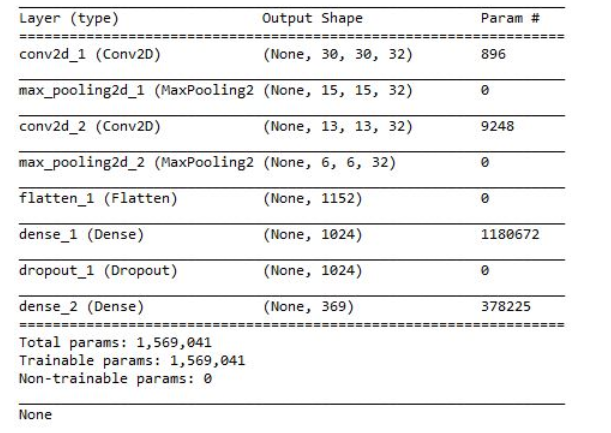
\includegraphics[width=1\textwidth]{figures/andi/p10.PNG}}
	\caption{In[10]}
\end{figure}

\item Jelaskan kode program pada blok \# In[11]
\par Berikut adalah kode program yang digunakan :
\lstinputlisting[firstline=89, lastline=90, caption=Kode Program 11, label={11}]{src/1164064/MathSymbols.py}
\par Dari kode listing pada kode program 11, dapat dijelaskan seperti berikut :
\begin{itemize}
\item Impor Modul Callbacks dari Librari Keras.
\item Variabel callback mendefinisikan Callback ini untuk menulis log untuk TensorBoard, yang memungkinkan Anda untuk memvisualisasikan grafik dinamis dari pelatihan dan metrik pengujian Anda, serta histogram aktivasi untuk berbagai lapisan dalam model Anda.
\end{itemize}
\par Sehingga dari kode program tersebut bila dijalankan, maka menghasilkan seperti pada gambar 
\begin{figure}[!htbp]
	\centerline{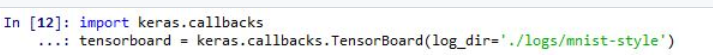
\includegraphics[width=1\textwidth]{figures/andi/p11.PNG}}
	\caption{In[11]}
\end{figure}

\item Jelaskan kode program pada blok \# In[12]
\par Berikut adalah kode program yang digunakan :
\lstinputlisting[firstline=93, lastline=102, caption=Kode Program 12, label={12}]{src/1164064/MathSymbols.py}
\par Dari kode listing pada kode program 12, dapat dijelaskan seperti berikut :
\begin{itemize}
\item Melakukan fit model dengan 32 ukuran subset dari sampel pelatihan Anda
\item Epoch sebanyak 10 kali
\item Vebrose=2 maksudnya menampilkan nomor dari epoch yang sedang berjalan atau yang sudah dijalankan.
\item Validasi plit sebanayk 20\% sebagai fraksi data pelatihan untuk digunakan sebagai data validasi.
\item Menggunakan TensorBoard sebagai callback untuk diterapkan selama pelatihan dan validasi.
\item Variabel score mengembalikan nilai evaluate untuk menampilkan data lost dan data accuracy dari test
\item Menampilkan data loss dengan menghitung jumlah kemunculan nol .
\item Menampilkan data accuracy dengan menghitung jumlah kemunculan 1.
\end{itemize}
\par Sehingga dari kode program tersebut bila dijalankan, maka menghasilkan seperti pada gambar 
\begin{figure}[!htbp]
	\centerline{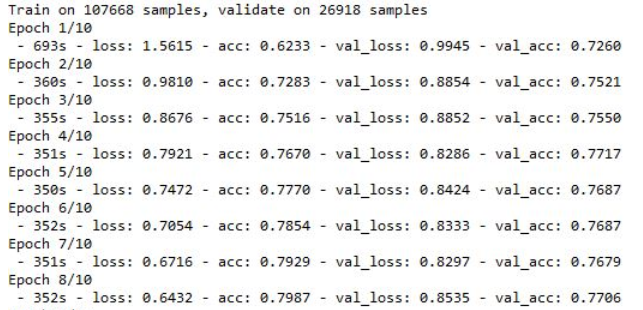
\includegraphics[width=1\textwidth]{figures/andi/p12.PNG}}
	\caption{In[12]}
\end{figure}

\item Jelaskan kode program pada blok \# In[13]
\par Berikut adalah kode program yang digunakan :
\lstinputlisting[firstline=106, lastline=137, caption=Kode Program 13, label={13}]{src/1164064/MathSymbols.py}
\par Dari kode listing pada kode program 13, dapat dijelaskan seperti berikut :
\begin{itemize}
\item impor modul time dari python anaconda
\item Variabel result berisikan array kosong.
\item Menggunakan convolution 2D yang dimana akan memiliki 1 atau 2 layer.
\item Mendefinisikan dense\_size dengan ukuran 128, 256, 512, 1024, 2048
\item Mendefinsikan drop\_out dengan 0, 25\%, 50\%, dan 75\%
\item Melakukan pemodelan Sequential
\item Jika ini adalah layer pertama, kita perlu memasukkan bentuk input.
\item Kalau tidak kita hanya akan menambahkan layer.
\item Kemudian, setelah menambahkan layer konvolusi, kita akan melakukan hal yang sama dengan max pooling.
\item  Lalu, kita akan meratakan atau flatten dan menambahkandense size ukuran apa pun yang berasal dari dense\_size. Dimana akan selalu menggunakan algoritma tanh
\item Jika dropout digunakan, kita akan menambahkan layer dropout. Menyebut dropout ini berarti, katakanlah 50\%, bahwa setiap kali ia memperbarui bobot setelah setiap batch, ada peluang 50\% untuk setiap bobot yang tidak akan diperbarui
\item menempatkan ini di antara dua lapisan padat untuk dihidupkan dari melindunginya dari overfitting.
\item  Lapisan terakhir akan selalu menjadi jumlah kelas karena itu harus, dan menggunakan softmax. Itu dikompilasi dengan cara yang sama.
\item Atur direktori log yang berbeda untuk TensorBoard sehingga dapat membedakan konfigurasi yang berbeda.
\item Variabel start akan memanggil modul time atau waktu
\item Melakukan fit atau compile 
\item MElakukan scoring dengan .evaluate yang akan menampilkan data loss dan accuracy dari model
\item end merupakan variabel untuk melihat waktu akhir pada saat pemodelan berhasil dilakukan.
\item Menampilkan hasil dari run skrip diatas
\end{itemize}
\par Sehingga dari kode program tersebut bila dijalankan, maka menghasilkan seperti pada gambar 
\begin{figure}[!htbp]
	\centerline{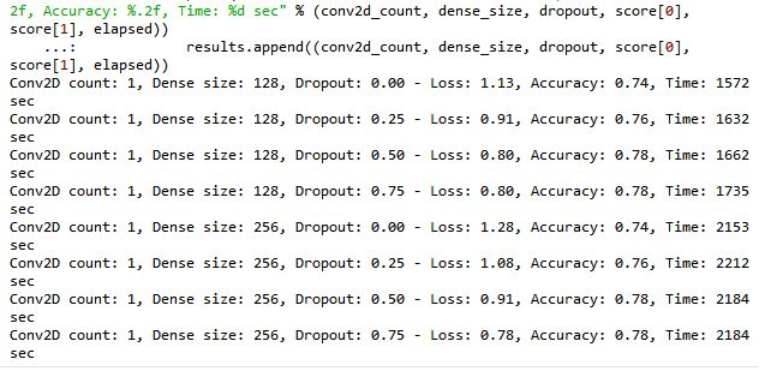
\includegraphics[width=1\textwidth]{figures/andi/p13.PNG}}
	\caption{In[13]}
	
\end{figure}
\item Jelaskan kode program pada blok \# In[14]
\par Berikut adalah kode program yang digunakan :
\lstinputlisting[firstline=141, lastline=151, caption=Kode Program 14, label={14}]{src/1164064/MathSymbols.py}
\par Dari kode listing pada kode program 14, dapat dijelaskan seperti berikut :
\begin{itemize}
\item Melakukan pemodelan Sequential
\item Untuk layer pertama, Menambahkan Convolutio 2D dengan dmensi 32, dan ukuran matriks 3x3 dengan function aktivasi yang digunakan yaitu relu dan menampilkan input\_shape
\item Dilakukan Max Pooling 2D dengan ukuran matriks 2x2
\item Untuk layer kedua, melakukan Convolusi lagi dengan kriteria yang sama tanpa menambahkan input, ini dilakukan untuk mendapatkan data yang terbaik
\item Flatten digubakan ntuk meratakan inputan
\item Menambahkan dense input sebanyak 128 neuron dengan menggunakan function aktivasi tanh.
\item Dropout sebanyak 50\% untuk menghindari overfitting
\item Menambahkan dense pada model untuk output dimana layer ini akan menjadi jumlah dari class yang ada.
\item Mengcompile model yang didefinisikan diatas
\item Menampilkan ringkasan dari pemodelan yang dilakukan
\end{itemize}
\par Sehingga dari kode program tersebut bila dijalankan, maka menghasilkan seperti pada gambar 
\begin{figure}[!htbp]
	\centerline{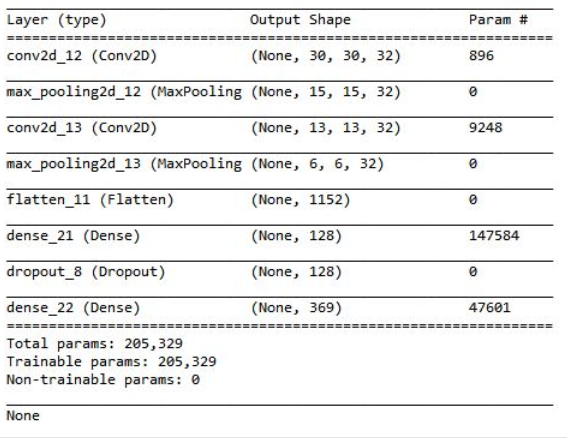
\includegraphics[width=1\textwidth]{figures/andi/p14.PNG}}
	\caption{In[14]}

\end{figure}
\item Jelaskan kode program pada blok \# In[15]
\par Berikut adalah kode program yang digunakan :
\lstinputlisting[firstline=153, lastline=155, caption=Kode Program 15, label={15}]{src/1164064/MathSymbols.py}
\par Dari kode listing pada kode program 15, dapat dijelaskan seperti berikut :
\begin{itemize}
\item Melakukan fit dengan join data train dan test agar dapat dilakukan pelatihan untuk jaringan pada smeua data yang dimiliki.
\end{itemize}
\par Sehingga dari kode program tersebut bila dijalankan, maka menghasilkan seperti pada gambar 
\begin{figure}[!htbp]
	\centerline{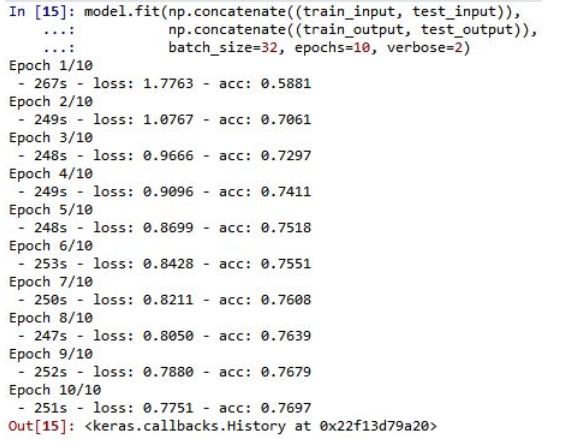
\includegraphics[width=1\textwidth]{figures/andi/p15.PNG}}
	\caption{In[15]}
	\end{figure}

\item Jelaskan kode program pada blok \# In[16]
\par Berikut adalah kode program yang digunakan :
\lstinputlisting[firstline=158, lastline=158, caption=Kode Program 16, label={16}]{src/1164064/MathSymbols.py}
\par Dari kode listing pada kode program 16, dapat dijelaskan seperti berikut :
\begin{itemize}
\item Menyimpan atau save model yang telah di latih dengan nama mathsymbols.model 
\end{itemize}
\par Sehingga dari kode program tersebut bila dijalankan, maka menghasilkan seperti pada gambar 
\begin{figure}[!htbp]
	\centerline{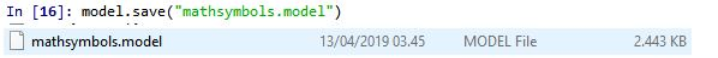
\includegraphics[width=1\textwidth]{figures/andi/p16.PNG}}
	\caption{In[16]}
\end{figure}

\item Jelaskan kode program pada blok \# In[17]
\par Berikut adalah kode program yang digunakan :
\lstinputlisting[firstline=161, lastline=161, caption=Kode Program 17, label={17}]{src/1164064/MathSymbols.py}
\par Dari kode listing pada kode program 17, dapat dijelaskan seperti berikut :
\begin{itemize}
\item Simpan label enkoder (untuk membalikkan one-hot encoder) dengan nama classes.npy
\end{itemize}
\par Sehingga dari kode program tersebut bila dijalankan, maka menghasilkan seperti pada gambar 
\begin{figure}[!htbp]
	\centerline{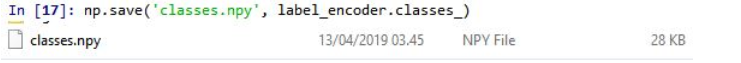
\includegraphics[width=1\textwidth]{figures/andi/p17.PNG}}
	\caption{In[17]}
\end{figure}

\item Jelaskan kode program pada blok \# In[18]
\par Berikut adalah kode program yang digunakan :
\lstinputlisting[firstline=167, lastline=169, caption=Kode Program 18, label={18}]{src/1164064/MathSymbols.py}
\par Dari kode listing pada kode program 18, dapat dijelaskan seperti berikut :
\begin{itemize}
\item Impor models dari librari Keras
\item Variabel model2 akan memanggil model yang telah disave tadi 
\item Menampilkan ringkasan dari hasil pemodelan
\end{itemize}
\par Sehingga dari kode program tersebut bila dijalankan, maka menghasilkan seperti pada gambar 
\begin{figure}[!htbp]
	\centerline{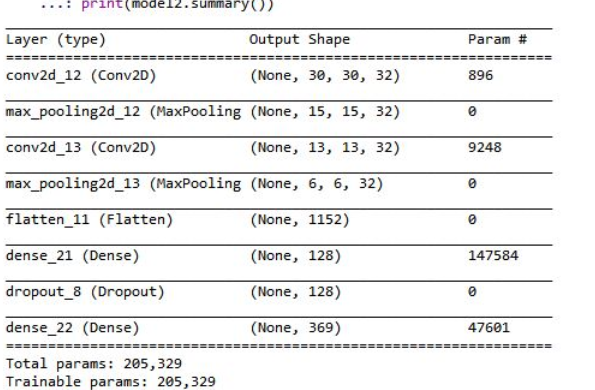
\includegraphics[width=1\textwidth]{figures/andi/p18.PNG}}
	\caption{In[18]}
\end{figure}

\item Jelaskan kode program pada blok \# In[19]
\par Berikut adalah kode program yang digunakan :
\lstinputlisting[firstline=172, lastline=184, caption=Kode Program 19, label={19}]{src/1164064/MathSymbols.py}
\par Dari kode listing pada kode program 19, dapat dijelaskan seperti berikut :
\begin{itemize}
\item Memanggil fungsi LabelEncoder
\item Variabel label\_encoder akan memanggil class yang disave sebelumnya.
\item Function Predict akan mengubah gambar kedalam bentuk array
\item Variabel prediction akan melakukan prediksi untuk model2 dengan reshape variabel newimg dengan bentukarray 4D.
\item Variabel inverted akan mencari nilai tertinggi output dari hasil prediksi tadi
\item Menampilkan hasil dari variabel prediction dan inverted
\end{itemize}
\par Sehingga dari kode program tersebut bila dijalankan, maka menghasilkan seperti pada gambar 
\begin{figure}[!htbp]
	\centerline{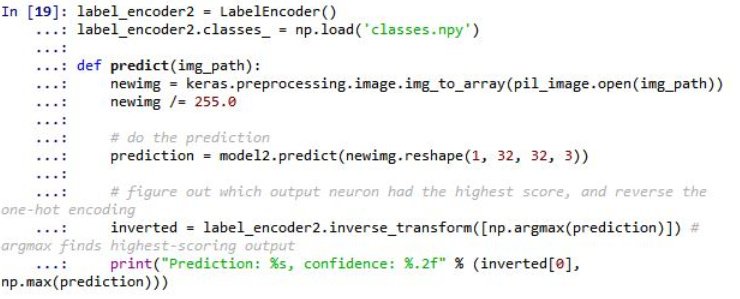
\includegraphics[width=1\textwidth]{figures/andi/p19.PNG}}
	\caption{In[19]}
\end{figure}

\item Jelaskan kode program pada blok \# In[20]
\par Berikut adalah kode program yang digunakan :
\lstinputlisting[firstline=187, lastline=191, caption=Kode Program 20, label={20}]{src/1164064/MathSymbols.py}
\par Dari kode listing pada kode program 20, dapat dijelaskan seperti berikut :
\begin{itemize}
\item Melakukan prediksi dari pelatihan dari gambar v2-00010.png
\item Melakukan prediksi dari pelatihan dari gambar v2-00500.png
\item Melakukan prediksi dari pelatihan dari gambar v2-00700.png
\end{itemize}
\par Sehingga dari kode program tersebut bila dijalankan, maka menghasilkan seperti pada gambar 
\begin{figure}[!htbp]
	\centerline{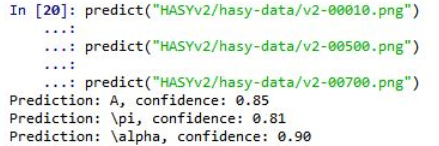
\includegraphics[width=1\textwidth]{figures/andi/p20.PNG}}
	\caption{In[20]}
\end{figure}
\end{enumerate}

\subsection{Penanganan Eror}
\begin{enumerate}
\item skrinsut error
\begin{figure}[!htbp]
	\centerline{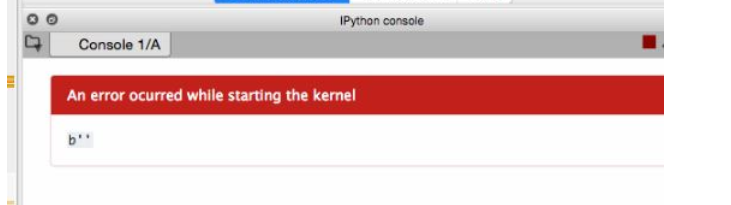
\includegraphics[width=1\textwidth]{figures/andi/p21.PNG}}
	\caption{Eror}
\end{figure}

\item Tuliskan kode eror dan jenis errornya
\subitem Eror tersebut merupakan eror yang terjadi dan membuat kita tidak dapat mengakses dan menggunakan kernel atau konsol pada spyder.
\item Solusi pemecahan masalah error tersebut
\begin{itemize}
\item Tutup spyder yang sedang dijalankan
\item Kemudian buka kembali spyder
\item maka eror pada kernel tersebut akan hilang dan kembali stabil agar bisa mengakses konsol tersebut.
\end{itemize}
\end{enumerate}


\section{Aip Suprapto Munari-1164063}
\subsection{Teori}
\begin{enumerate}
\item Kenapa File Suara Harus Dilakukan Tokenizer
\begin{itemize}
\item Penjelasan: Untuk membedakan karakter-karakter tertentu dalam suatu teks dan juga sebagai pemisah kata atau bukan.Tokenizer dilakukan dengan cara melakukan pemotongan string input berdasarkan tiap kata yang menyusunnya.
\par 
\par
\item Ilustrasi Gambar
\item Tokenizer \ref{teori1}
\begin{figure}[!hbtp]
\centering
\includegraphics[scale=0.7]{figures/AIP/g1.PNG}
\caption{Tokenizer Aip}
\label{teori1}
\end{figure}
\par
\end{itemize}
\par
\par

\item Jelaskan konsep dasar K Fold Cross Validation pada dataset komentar Youtube pada kode listing 
\lstinputlisting{src/1164063/chapter7-2.py}
\begin{itemize}
\item Penjelasan: Startified KFold berisikan presentasi sampel untuk setiap kelas. Dimana dalam ilustrasi ini sampel dibagi menjadi 5 dalam setiap class nya. Kemudian sampel tadi akan dimasukan kedalam class dari dataset youtube tadi.
\par 
\par
\item Ilustrasi Gambar
\item K-Fold Cross Validation \ref{teori2}
\begin{figure}[!hbtp]
\centering
\includegraphics[scale=0.7]{figures/AIP/g2.PNG}
\caption{K-Fold Cross Validation Aip}
\label{teori2}
\end{figure}
\par
\end{itemize}
\par
\par

\item Jelaskan apa maksudnya kode program for train, test in splits.dilengkapi dengan ilustrasi atau gambar.
\begin{itemize}
\item Penjelasan: Maksudnya yaitu untuk menguji apakah setiap data pada dataset sudah di split dan tidak terjadi penumpukan. Yang dimana maksudnya di setiap class tidak akan muncul id yang sama. Ilustrasinya misalkan kita memiliki 4 botol minuman dengan model yang berbeda. Kemudian kita bagikan kedua anak, tentunya setiap anak yang menerima botol tidak memiliki botol minuman  yang sama modelnya.
\par 
\par
\item Ilustrasi Gambar
\item No 3  \ref{teori3}
\begin{figure}[!hbtp]
\centering
\includegraphics[scale=0.2]{figures/AIP/g3.PNG}
\caption{No 3 Aip}
\label{teori3}
\end{figure}
\par
\end{itemize}
\par
\par

\item Jelaskan apa maksudnya kode program {train\_content = d['CONTENT'].iloc[train\_idx]} dan {test\_content = d['CONTENT'].iloc[test\_idx]}.
\begin{itemize}
\item Penjelasan: Maksudnya yaitu mengambil data pada kolom atau index CONTENT yang merupakan bagian dari train\_idx dan test\_idx. Ilustrasinya, ketika data telah diubah menjadi train dan test maka kita dapat memilihnya untuk ditampilkan pada kolom yang diinginkan.
\par 
\par
\item Ilustrasi Kalimat :
\par Jika dicontohkan dengan sebuah penjelasan maka bisa dikatakan apabila index CONTENT tersebut direalisasikan maka untuk data yang telah diubah menjadi training data maupun test data bisa dipilih kolom ataupun nilai apa yang akan ditampilkan dan dieksekusi sesuai dengan kebetuhan ataupun keinginan.
\end{itemize}
\par
\par

\item Jelaskan apa maksud dari fungsi tokenizer {tokenizer = Tokenizer(num\_words=2000)} dan tokenizer.{tokenizer.fit\_on\_texts(train\_content)}, dilengkapi dengan ilustrasi atau gambar.
\begin{itemize}
\item Penjelasan: Dimana variabel tokenizer akan melakukan vektorisasi kata menggunakan fungsi Tokenizer yang dimana jumlah kata yang ingin diubah kedalam bentuk token adalah 2000 kata. Dan untuk \emph{tokenizer.fit\_on\_texts(train\_content)} maksudnya kita akan melakukan fit tokenizer hanya untuk data trainnya saja tidak dengan data test nya untuk kolom CONTENT. 
\par 
\par
\item Ilustrasi Gambar
\item No 5 \ref{teori5}
\begin{figure}[!hbtp]
\centering
\includegraphics[scale=0.4]{figures/AIP/g5.PNG}
\caption{No 5 Aip}
\label{teori5}
\end{figure}
\par
\end{itemize}
\par
\par


\item Jelaskan apa maksud dari fungsi \emph{d\_train\_inputs = tokenizer.texts\_to\_matrix(train\_content, mode='tfidf')} dan \emph{d\_test\_inputs = tokenizer.texts\_to\_matrix(test\_content, mode='tfidf')}, dilengkapi dengan ilustrasi kode dan atau gambar.
\begin{itemize}
\item Penjelasan: Maksudnya yaitu untuk variabel d\_train\_inputs akan melakukan tokenizer dari bentuk teks ke matrix dari data train\_content dengan mode matriksnya yaitu tf-idf begitu juga dengan variabel d\_test\_inputs untuk data test. Berikut gambar ilustrasinya
\par 
\par
\item Ilustrasi Gambar
\item No 6 \ref{teori6}
\begin{figure}[!hbtp]
\centering
\includegraphics[scale=0.3]{figures/AIP/g6.PNG}
\caption{No 6 Aip}
\label{teori6}
\end{figure}
\par
\end{itemize}
\par
\par

\item Jelaskan apa maksud dari fungsi \emph{d\_train\_inputs = d\_train\_inputs/np.amax(np.absolute(d\_train\_inputs))} dan \emph{d\_test\_inputs = d\_test\_inputs/np.amax(np.absolute(d\_test\_inputs))}, dilengkapi dengan ilustrasi atau gambar.
\begin{itemize}
\item Penjelasan: Fungsi tersebut akan membagi matrix tf-idf tadi dengan amax yaitu mengembalikan maksimum array atau maksimum sepanjang sumbu. Yang hasilnya akan dimasukan kedalam variabel d\_train\_inputs untuk data train dan d\_test\_inputs untuk data test dengan nominal absolut atau tanpa ada bilangan negatif dan koma.
\par 
\par
\item Ilustrasi Gambar
\item No 7 \ref{teori7}
\begin{figure}[!hbtp]
\centering
\includegraphics[scale=0.4]{figures/AIP/g7.PNG}
\caption{No 7 Aip}
\label{teori7}
\end{figure}
\par
\end{itemize}
\par
\par

\item Jelaskan apa maksud fungsi dari d\_train \_outputs = np\_utils.to\_categorical(d['CLASS'].iloc[train dan d\_test \_outputs = np\_ utils.to\_categorical(d['CLASS'].iloc[test\_idx]) dalam kode program
\begin{itemize}
\item Penjelasan: Dari fungsi pada kode program tersebut dijelaskan fungsi tersebut ditujukan untuk melakukan one-hot encoding agar dapat masuk dan digunakan di neural network. One-hot encoding diambil dari 'CLASS' yang berarti hanya terdapat 2 neuron, yaitu satu nol(1,0) atau nol satu(0,1) karena pilihannya hanya ada dua (spam atau bukan).
\par 
\par
\item Ilustrasi Gambar
\item No 8 \ref{teori8}
\begin{figure}[!hbtp]
\centering
\includegraphics[scale=0.4]{figures/AIP/g8.PNG}
\caption{No 8 Aip}
\label{teori8}
\end{figure}
\par
\end{itemize}
\par
\par

\item Jelaskan apa maksud dari fungsi di listing!
\lstinputlisting{src/1164063/chapter7-9.py}
\begin{itemize}
\item Penjelasan: Dari fungsi pada kode program tersebut ditujukan untuk melakukan pemodelan dengan sequential, membandingkan setiap satu larik elemen dengan cara satu persatu secara beruntun. Dimana terdapat 512 neuron inputan dengan input shape 2000 vektor. Lalu model dilakukan aktivasi dengan fungsi 'relu'. Kemudian dilakukan pemotongan bobot supaya tidak overfitting sebesar 50 persen dari neuron inputan 512. Lalu pada layer output terdapat 2 neuron outputan yaitu nol(1,0) atau nol satu(0,1). Kemudian outputan tersebut diaktivasi menggunakan fungsi softmax.
\par 
\end{itemize}
\par
\par

\item Jelaskan apa maksud dari fungsi di listing!
\lstinputlisting{src/1164063/chapter7-10.py}
\begin{itemize}
\item Penjelasan: Dari fungsi pada kode program tersebut model yang telah dibuat selanjutnya dicompile dengan menggunakan algoritma optimisasi dengan fungsi-fungsi loss, fungsi opttimaizer dan fungsi metrik. Dimana nama masing-masing fungsi tersebut adalah categorical\_crossentropy, adamax dan accuracy.
\par 
\end{itemize}
\par
\par

\item 	Apa Itu Deep Learning
\begin{itemize}
\item Penjelasan: 
\par  Deep learning merupakan sub bidang pembelajaran mesin yang berkaitan dengan algoritma.
\end{itemize}
\par
\par

\item Apa itu Deep Neural Network Dan Apa Bedanya Dengan Deep Learning :
\begin{itemize}
\item Penjelasan Deep Neural Network : 
\par  Deep neural network adalah jaringan syaraf dengan tingkat kompleksitas tertentu, jaringan syaraf dengan lebih dari dua lapisan.
\par
\item Perbedaan Deep Neural Network Dan Deep Learning :
\par  Perbedaan antara deep neural network dan deep learning terletak pada kedalaman model. deep learning adalah frasa yang digunakan untuk jaringan saraf yang kompleks. Kompleksitas ini disebabkan oleh pola yang rumit tentang bagaimana informasi dapat mengalir di seluruh model. Arsitekturnya menjadi lebih kompleks tetapi konsep deep learning masih sama. Meskipun sekarang ada peningkatan jumlah layer dan node tersembunyi yang terintegrasi untuk memperkirakan output.
\end{itemize}
\par
\par

\item Bagaimana Perhitungan Algoritma Dengan Ukuran Stride (NPM mod3+1)x(NPM mod3+1) Yang  Terdapat Pada Max Pooling :
\begin{itemize}
\item Penjelasan :
\par Konvolusi pada sebuah gambar dilakukan dalam image processing untuk menerapkan operator yang mempunyai nilai output dari piksel gambar yang berasal dari kombinasi linear nilai input piksel tertentu pada gambar.
\par
\item Langkah-langkah Algoritma Konvulasi Sesuai NPM : \ref{chapter-7-algoritma-konvolusi-Aip}
\par
\par
\begin{figure}[!hbtp]
\centering
\includegraphics[scale=0.52]{figures/AIP/g13.PNG}
\caption{Langkah Algoritma Konvolusi Berdasarkan NPM- Aip}
\label{chapter-7-algoritma-konvolusi-Aip}
\end{figure}
\par
\par
\end{itemize}
\end{enumerate}

\begin{itemize}
\item  Plagiarisme Aip: \ref{plagiarisme-Aip}
\par
\begin{figure}[!hbtp]
\centering
\includegraphics[scale=0.3]{figures/AIP/plagiat.PNG}
\caption{Plagiarisme- Aip}
\label{chapter-7-plagiarisme-Aip}
\end{figure}
\par
\par
\end{itemize}


\par
\par
\subsection{Praktek}
\begin{enumerate}
\item Jelaskan kode program pada blok \# In[1].
\begin{itemize}
\item Kode Program:
\lstinputlisting[firstline=1, lastline=19, caption=Praktek1.py, label={lst:import}]{src/1164063/chapter7-praktikum-1-aip.py}
\par Hasil \ref{in1aip} :
\begin{figure}[!hbtp]
\centering
\includegraphics[scale=0.7]{figures/AIP/prak1.PNG}
\caption{In 1 Aip}
\label{in1aip}
\end{figure}
\par Baris 1: Mengimpoer file csv.
\par Baris 2: Dari library PIL impor gambar sebagai pil\_image.
\par Baris 3: Impor fungsi fungsi keras.processing.image
\end{itemize}
\par

\item Jelaskan kode program pada blok \# In[2].
\begin{itemize}
\item Kode Program:
\lstinputlisting[firstline=1, lastline=19, caption=Praktek2.py, label={lst:import}]{src/1164063/chapter7-praktikum-2-aip.py}
\par Hasil \ref{in2aip} :
\begin{figure}[!hbtp]
\centering
\includegraphics[scale=0.7]{figures/AIP/prak2.PNG}
\caption{In 2 Aip}
\label{in2aip}
\end{figure}
\par Baris 1: Membuat variabel images tanpa parameter, karena di dalam kurung kosong tanpa ada parameter yang diisi.
\par Baris 2: Membuat variabel class tanpa parameter juga karna tiada ada parameter di dalam kurung.
\par Baris 3: Membuka file HASYv2/hasy-data-labels.csv sebagai csvfile.
\par Baris 4: Membuat variabel csvreader yang memfungsikan pembacaan dari file csv yang dimasukkan
\par Baris 5: Membuat variabel i dengan parameter 0
\par Baris 6: Mengeksekusi data dari baris di pembacaan file csv.
\par Baris 7: Menggunakan perintah "if" dengan ketentuan variabel i lebih besar dari  0.
\par Baris 8: Membuat variabel img dengan nama keras.processing yang mengubah image menjadi bentuk array (bilangan) dari file HASYv2 yang dibuka dengan row berparameter 0.
\par Baris 9: Membuat variabel img tidak sama dengan 255.0
\par Baris 10: Mendefinisikan fungsi imgs.append dimana merupakan proses menggabungkan data dengan file lain  yang ditentukan dengan 3 parameter yaitu row[0], row[2] dan variabel img.
\par Baris 11: Mendefinisikan fungsi append kembali dari variabel classes dengan parameternya row[2].
\par Baris 12: Mendefinisikan fungsi dimana i variabel i akan ditambah nilainya sehingga akan bernilai 1 ( Contoh nilai i=0 dengan adanya penambahan maka hasilnya akan menjadi 1 )
\end{itemize}
\par


\item Jelaskan kode program pada blok \# In[3].
\begin{itemize}
\item Kode Program:
\lstinputlisting[firstline=1, lastline=19, caption=Praktek3.py, label={lst:import}]{src/1164063/chapter7-praktikum-3-aip.py}
\par Hasil \ref{in3aip} :
\begin{figure}[!hbtp]
\centering
\includegraphics[scale=0.7]{figures/AIP/prak3.PNG}
\caption{In 3 Aip}
\label{in3aip}
\end{figure}
\par Baris 1: Import modul random
\par Baris 2: Melakukan pengocokan terhadap modul dengan parameter dimana variabelnya imgs
\par Baris 3: Membagi dan memecah index dalam bentuk integer dengan mengkalikan nilai 0.8 dengan fungsi len yang mengembalikan jumlah item dari variabel imgs.
\par Baris 4: Membuat variabel train yang mengeksekusi imgs dengan pemecahan index pada data awa.l
\par Baris 5: Membuat variabel test yang mengeksekusi imgs dengan pemecahan index pada dataakhir.

\end{itemize}
\par

\item Jelaskan kode program pada blok \# In[4].
\begin{itemize}
\item Kode Program:
\lstinputlisting[firstline=1, lastline=19, caption=Praktek4.py, label={lst:import}]{src/1164063/chapter7-praktikum-4-aip.py}
\par Hasil \ref{in4aip} :
\begin{figure}[!hbtp]
\centering
\includegraphics[scale=0.7]{figures/AIP/prak4.PNG}
\caption{In 4 Aip}
\label{in4aip}
\end{figure}
\par Baris 1: Import library numpy sebagai np.
\par Baris 2: Membuat variabel train\_input dimana mengubah input menjadi sebuah array dari np dengan menggunakan fungsi list untuk mengkoleksikan data yang dipilih dan dapat diubah. Didalamnya diterapkan fungsi map untuk mengembalikan iterator dari datanya dengan memfungsikan lamda pada row dengan parameter [2] untuk membuat objek fungsi menjadi lebih kecil dan mudah dieksekusi dari variabel train.
\par Baris 3:Membuat variabel test\_input dengan fungsi yang sama seperti train\_input yang membedakan hanya datanya / inputan yang diproses berasal dari variabel test
\par Baris 4: Membuat variabel train\_output dimana mengubah keluaran menjadi sebuah array dari np dengan menggunakan fungsi list untuk mengkoleksikan data yang dipilih dan dapat diubah. Didalamnya diterapkan fungsi map untuk mengembalikan iterator dari datanya dengan memfungsikan lamda pada row dengan parameter[1] untuk membuat objek fungsi menjadi lebih kecil dan mudah dieksekusi dari variabel train.
\par Baris 5: Membuat variabel test\_output dengan fungsi yang sama seperti train\_output yang membedakan hanya datanya / inputan yang diproses berasal dari variabel test
\end{itemize}
\par

\item Jelaskan kode program pada blok \# In[5].
\begin{itemize}
\item Kode Program:
\lstinputlisting[firstline=1, lastline=19, caption=Praktek5.py, label={lst:import}]{src/1164063/chapter7-praktikum-5-aip.py}
\par Hasil \ref{in5aip} :
\begin{figure}[!hbtp]
\centering
\includegraphics[scale=0.7]{figures/AIP/prak5.PNG}
\caption{In 5 Aip}
\label{in5aip}
\end{figure}
\par Baris 1: Import labelEncoder dari sklearn.processing digunakan untuk menormalkan label dimana label encoder hanya didefinisikan dengan nilai antara 0 dan n\_classes-1.
\par Baris 2: Memasukkan modul / fungsi OneHotEncoder dari sklearn.processing yang digunakan untuk mendefinisikan fitur input dimana mengambil nilai dalam kisaran [0, maks (nilai)).
\end{itemize}
\par

\item Jelaskan kode program pada blok \# In[6].
\begin{itemize}
\item Kode Program:
\lstinputlisting[firstline=1, lastline=19, caption=Praktek5.py, label={lst:import}]{src/1164063/chapter7-praktikum-6-aip.py}
\par Hasil \ref{in6aip} :
\begin{figure}[!hbtp]
\centering
\includegraphics[scale=0.7]{figures/AIP/prak6.PNG}
\caption{In 6 Aip}
\label{in6aip}
\end{figure}
\par Baris 1: Membuat variabel label\_encoder dengan penerapan modul / fungsi dari LabelEncoder tanpa parameter
\par Baris 2: Membuat variabel integer\_encoded dengan penerapan fungsi label\_encoder.fit\_transform (ekstrasi fitur object ) dari variabel classes dimana akan mengembalikan beberapa data yang diubah kembali dari variabel label\_encoder.
\end{itemize}
\par

\item Jelaskan kode program pada blok \# In[7].
\begin{itemize}
\item Kode Program:
\lstinputlisting[firstline=1, lastline=19, caption=Praktek7.py, label={lst:import}]{src/1164063/chapter7-praktikum-7-aip.py}
\par Hasil \ref{in7aip} :
\begin{figure}[!hbtp]
\centering
\includegraphics[scale=0.7]{figures/AIP/prak7.PNG}
\caption{In 7 Aip}
\label{in7aip}
\end{figure}
\par Baris 1: Membuat variabel onehot\_encoder yang memanggil fungsi OneHotEncoder tanpa mengembalikan matriks karena sparse=false.
\par Baris 2: Membuat variabel integer\_encoded memanggil variabel integer\_encoded pada kode program 6 untuk dieksekusi memberikan bentuk baru ke array tanpa mengubah datanya dari mengembalikan panjang nilai dari integer\_encoded.
\par Baris 3: Onehotencoding melakukan fitting pada integer\_encoded.
\end{itemize}
\par

\item Jelaskan kode program pada blok \# In[8].
\begin{itemize}
\item Kode Program:
\lstinputlisting[firstline=1, lastline=19, caption=Praktek8.py, label={lst:import}]{src/1164063/chapter7-praktikum-8-aip.py}
\par Hasil \ref{in8aip} :
\begin{figure}[!hbtp]
\centering
\includegraphics[scale=0.7]{figures/AIP/prak8.PNG}
\caption{In 8 Aip}
\label{in8aip}
\end{figure}
\par Baris 1: Membuat variabel train\_output\_int yang mengeksekusi label\_encoder dengan mengubah nilai dari parameter variabel train\_output.
\par Baris 2: Membuat variabel train\_output yang mengeksekusi variabel onehot\_encoder dari kode program 7 dengan mengubah nilai dari variabel parameter train\_output\_int yang datanya sudah diubah kedalam bentuk array dan panjang nilai dari train\_output\_int telah dikembalikan.
\par Baris 3: Membuat variabel test\_output\_int yang mengeksekusi label\_encoder dengan mengubah nilai dari parameter variabel test\_output.
\par Baris 4: Membuat variabel test\_output yang mengeksekusi variabel onehot\_encoder dari kode program 7 dengan mengubah nilai dari variabel parameter test\_output\_int yang datanya sudah diubah kedalam bentuk array dan panjang nilai dari test\_output\_int telah dikembalikan.
\par Baris 5: Membuat variabel num\_classes untuk mengetahui jumlah class dari lebel\_encoder
\par Baris 6: Perintah print digunakan untuk memunculkan hasil dari variabel num\_classes
\end{itemize}
\par

\item Jelaskan kode program pada blok \# In[9].
\begin{itemize}
\item Kode Program:
\lstinputlisting[firstline=1, lastline=19, caption=Praktek9.py, label={lst:import}]{src/1164063/chapter7-praktikum-9-aip.py}
\par Hasil \ref{in9aip} :
\begin{figure}[!hbtp]
\centering
\includegraphics[scale=0.7]{figures/AIP/prak9.PNG}
\caption{In 9 Aip}
\label{in9aip}
\end{figure}
\par Baris 1: Memanggil atau melakukan importing fungsi model sequential dari library keras.
\par Baris 2: Memanggil atau melakukan importing fungsi layer dense, dropout, dan flatten dari library keras.
\par Baris 3: Memanggil atau melakukan importing fungsi layer Conv2D dan MaxPooling2D dari library keras.
\end{itemize}
\par

\item Jelaskan kode program pada blok \# In[10].
\begin{itemize}
\item Kode Program:
\lstinputlisting[firstline=1, lastline=19, caption=Praktek10.py, label={lst:import}]{src/1164063/chapter7-praktikum-10-aip.py}
\par Hasil \ref{in10aip} :
\begin{figure}[!hbtp]
\centering
\includegraphics[scale=0.7]{figures/AIP/prak10.PNG}
\caption{In 10 Aip}
\label{in10aip}
\end{figure}
\par Baris 1: Melakukan pemodelan Sequential.
\par Baris 2: Menambahkan Konvolusi 2D dengan 32 filter konvolusi masing-masing berukuran 3x3 dengan algoritam activation relu dengan data dari train input mulai dari baris nol.
\par Baris 3: Menambahkan Max Pooling dengan matriks 2x2.
\par Baris 4: Penambahan Konvolusi 2D dengan 32 filter, konvolusi masing-masing berukuran 3x3 dengan algoritam activation relu.
\par Baris 5 Menambahkan Max Pooling dengan matriks 2x2.
\par Baris 6: Mendefinisikan inputan dengan 1024 neuron dan menggunakan algoritma tanh untuk activationnya.
\par Baris 7: Dropout terdiri dari pengaturan secara acak tingkat pecahan unit input ke 0 pada setiap pembaruan selama waktu pelatihan, yang membantu mencegah overfitting sebesar 50\% .
\par Baris 8: Untuk output layer menggunakan data dari variabel num classes dengan fugsi activationnya softmax.
\par Baris 9: Konfigurasi proses pembelajaran, melalui metode compile, sebelum melatih suatu model.
\par Baris 10: Menampilkan model yang telah dibuat.
\end{itemize}
\par

\item Jelaskan kode program pada blok \# In[11].
\begin{itemize}
\item Kode Program:
\lstinputlisting[firstline=1, lastline=19, caption=Praktek11.py, label={lst:import}]{src/1164063/chapter7-praktikum-11-aip.py}
\par Hasil \ref{in11aip} :
\begin{figure}[!hbtp]
\centering
\includegraphics[scale=0.7]{figures/AIP/prak11.PNG}
\caption{In 11 Aip}
\label{in11aip}
\end{figure}
\par Baris 1: Memasukkan / Mengimport library keras.callbacks dimana digunakan dalam penulisan log untuk TensorBoard, yang memungkinkan untuk memvisualisasikan grafik dinamis dari pelatihan dan metrik pengujian.
\par Baris 2: Membuat variabel tenserboard yang mendefinisikan fungsi TensorBoard pada keras.callbacks yang digunakan sebagai alat visualisasi yang disediakan dengan TensorFlow. Kemudian untuk fungsi log\_dir (jalur direktori tempat menyimpan file log yang akan diuraikan oleh TensorBoard) memanggil data yaitu './logs/mnist-style'
\end{itemize}
\par

\item Jelaskan kode program pada blok \# In[12].
\begin{itemize}
\item Kode Program:
\lstinputlisting[firstline=1, lastline=19, caption=Praktek12.py, label={lst:import}]{src/1164063/chapter7-praktikum-12-aip.py}
\par Hasil \ref{in12aip} :
\begin{figure}[!hbtp]
\centering
\includegraphics[scale=0.7]{figures/AIP/prak12.PNG}
\caption{In 12 Aip}
\label{in12aip}
\end{figure}
\par Baris 1: Menerapkan fungsi model.fit yang didalamnya memproses train\_input, train\_output
\par Baris 2: Selanjutnya pada penerapan fungsi yang sama difungsikan batch\_size ( jumlah sampel per pembaharuan sampel dari data yang diolah) apabila batch\_sizenya tidak ditemukan maka otomatis akan dijadikan nilai 32	
\par BAris 3: Pada penerapan fungsi yang sama, difungsikan epochs dimana perulangan dari berapa kali nilai yang digunakan untuk data, dan jumlahnya ialah 10
\par Baris 4: Mendefinisikan fungsi verbose dimana digunakan sebagai opsi untuk menghasilkan informasi logging dari data yang ditentukan dengan nilai 2
\par Baris 5: Mendefinisikan fungsi validation\_split untuk memecah nilai dari perhitungan validasinya sebesar 0,2. (Fraksi data pelatihan untuk digunakan sebagai data validasi)
\par Baris 6: Mendefinisikan fungsi callsbacks dengan parameternya yang mengeksekusi tensorboard dimana digunakan untuk visualisasikan parameter training, metrik, hiperparameter pada nilai/data yang diproses
\par Baris 7: Mendefinisikan variabel score dengan fungsi evaluate dari model yang ada dengan parameter test\_input, tst\_output dan verbose=2 dimana memprediksi output untuk input yang diberikan dan kemudian menghitung fungsi metrik yang ditentukan dalam modelnya
\item Baris 8: Mencetak score optimasi dari test dengan ketentuan nilai parameter 0
\item Baris 9: Mencetak score akurasi dari test dengan ketentuan nilai parameter 1
\end{itemize}
\par

\item Jelaskan kode program pada blok \# In[13].
\begin{itemize}
\item Kode Program:
\lstinputlisting[firstline=1, lastline=40, caption=Praktek13.py, label={lst:import}]{src/1164063/chapter7-praktikum-13-aip.py}
\par Hasil \ref{in13aip} :
\begin{figure}[!hbtp]
\centering
\includegraphics[scale=0.7]{figures/AIP/prak13.PNG}
\caption{In 13 Aip}
\label{in13aip}
\end{figure}
\par Baris 1: impor modul time dari python anaconda
\par Baris 2: Variabel result berisikan array kosong.
\par Baris 3: Menggunakan convolution 2D yang dimana akan memiliki 1 atau 2 layer.
\par Baris 4: Mendefinisikan dense\_size dengan ukuran 128, 256, 512, 1024, 2048
\par Baris 5: Mendefinsikan drop\_out dengan 0, 25\%, 50\%, dan 75\%
\par Baris 6:  Melakukan pemodelan Sequential
\par Baris 7: Jika ini adalah layer pertama, kita perlu memasukkan bentuk input.
\par Baris 8: Kalau tidak kita hanya akan menambahkan layer.
\par Baris 9: Kemudian, setelah menambahkan layer konvolusi, kita akan melakukan hal yang sama dengan max pooling.
\par Baris 10: Lalu, kita akan meratakan atau flatten dan menambahkandense size ukuran apa pun yang berasal dari dense\_size. Dimana akan selalu menggunakan algoritma tanh
\par Baris 11: Jika dropout digunakan, kita akan menambahkan layer dropout. Menyebut dropout ini berarti, katakanlah 50\%, bahwa setiap kali ia memperbarui bobot setelah setiap batch, ada peluang 50\% untuk setiap bobot yang tidak akan diperbarui
\par Baris 12: menempatkan ini di antara dua lapisan padat untuk dihidupkan dari melindunginya dari overfitting.
\par Lapisan terakhir akan selalu menjadi jumlah kelas karena itu harus, dan menggunakan softmax. Itu dikompilasi dengan cara yang sama.
\par Baris 13: Atur direktori log yang berbeda untuk TensorBoard sehingga dapat membedakan konfigurasi yang berbeda.
\par Baris 14: Variabel start akan memanggil modul time atau waktu
\par Baris 15: Melakukan fit atau compile 
\par Baris 16: Melakukan scoring dengan .evaluate yang akan menampilkan data loss dan accuracy dari model
\par Baris 17:  end merupakan variabel untuk melihat waktu akhir pada saat pemodelan berhasil dilakukan.
\par Baris 18:  Menampilkan hasil dari run skrip diatas 
\end{itemize}
\par

\item Jelaskan kode program pada blok \# In[14].
\begin{itemize}
\item Kode Program:
\lstinputlisting[firstline=1, lastline=19, caption=Praktek14.py, label={lst:import}]{src/1164063/chapter7-praktikum-14-aip.py}
\par Hasil \ref{in14aip} :
\begin{figure}[!hbtp]
\centering
\includegraphics[scale=0.7]{figures/AIP/prak14.PNG}
\caption{In 14 Aip}
\label{in14aip}
\end{figure}
\par Baris 1: Melakukan pemodelan Sequential
\par Baris 2: Untuk layer pertama, Menambahkan Convolutio 2D dengan dmensi 32, dan ukuran matriks 3x3 dengan function aktivasi yang digunakan yaitu relu dan menampilkan input\_shape
\par Baris 3: Dilakukan Max Pooling 2D dengan ukuran matriks 2x2
\par Baris 4:Untuk layer kedua, melakukan Convolusi lagi dengan kriteria yang sama tanpa menambahkan input, ini dilakukan untuk mendapatkan data yang terbaik
\par Baris 5:  Flatten digubakan ntuk meratakan inputan
\par Baris 6: Menambahkan dense input sebanyak 128 neuron dengan menggunakan function aktivasi tanh.
\par Baris 7: Dropout sebanyak 50\% untuk menghindari overfitting
\par Baris 8: Menambahkan dense pada model untuk output dimana layer ini akan menjadi jumlah dari class yang ada.
\par Baris 9: Mengcompile model yang didefinisikan diatas
\par Baris 10: Menampilkan ringkasan dari pemodelan yang dilakukan
\end{itemize}
\par

\item Jelaskan kode program pada blok \# In[15].
\begin{itemize}
\item Kode Program:
\lstinputlisting[firstline=1, lastline=19, caption=Praktek15.py, label={lst:import}]{src/1164063/chapter7-praktikum-15-aip.py}
\par Hasil \ref{in15aip} :
\begin{figure}[!hbtp]
\centering
\includegraphics[scale=0.7]{figures/AIP/prak15.PNG}
\caption{In 15 Aip}
\label{in15aip}
\end{figure}
\par Baris 1: Melakukan fit dengan join data train dan test agar dapat dilakukan pelatihan untuk jaringan pada semua data yang dimiliki.
\end{itemize}
\par

\item Jelaskan kode program pada blok \# In[16].
\begin{itemize}
\item Kode Program:
\lstinputlisting[firstline=1, lastline=19, caption=Praktek1.py, label={lst:import}]{src/1164063/chapter7-praktikum-16-aip.py}
\par Hasil \ref{in16aip} :
\begin{figure}[!hbtp]
\centering
\includegraphics[scale=0.7]{figures/AIP/prak16.PNG}
\caption{In 16 Aip}
\label{in16aip}
\end{figure}
\par Baris 1: Menyimpan atau save model yang telah di latih dengan nama mathsymbols.model 
\end{itemize}
\par

\item Jelaskan kode program pada blok \# In[17].
\begin{itemize}
\item Kode Program:
\lstinputlisting[firstline=1, lastline=19, caption=Praktek1.py, label={lst:import}]{src/1164063/chapter7-praktikum-17-aip.py}
\par Hasil \ref{in17aip} :
\begin{figure}[!hbtp]
\centering
\includegraphics[scale=0.7]{figures/AIP/prak17.PNG}
\caption{In 17 Aip}
\label{in17aip}
\end{figure}
\par Baris 1: Simpan label enkoder (untuk membalikkan one-hot encoder) dengan nama classes.npy
\end{itemize}
\par

\item Jelaskan kode program pada blok \# In[18].
\begin{itemize}
\item Kode Program:
\lstinputlisting[firstline=1, lastline=19, caption=Praktek18.py, label={lst:import}]{src/1164063/chapter7-praktikum-18-aip.py}
\par Hasil \ref{in18aip} :
\begin{figure}[!hbtp]
\centering
\includegraphics[scale=0.7]{figures/AIP/prak18.PNG}
\caption{In 18 Aip}
\label{in18aip}
\end{figure}
\par Baris 1: Impor models dari librari Keras
\par Baris 2: Variabel model2 akan memanggil model yang telah disave tadi 
\par Baris 3:  Menampilkan ringkasan dari hasil pemodelan
\end{itemize}
\par


\item Jelaskan kode program pada blok \# In[19].
\begin{itemize}
\item Kode Program:
\lstinputlisting[firstline=1, lastline=19, caption=Praktek19.py, label={lst:import}]{src/1164063/chapter7-praktikum-19-aip.py}
\par Hasil \ref{in19aip} :
\begin{figure}[!hbtp]
\centering
\includegraphics[scale=0.7]{figures/AIP/prak19.PNG}
\caption{In 19 Aip}
\label{in19aip}
\end{figure}
\item Menampilkan hasil dari variabel prediction dan inverted
\par Baris 1: Memanggil fungsi LabelEncoder
\par Baris 2: Variabel label\_encoder akan memanggil class yang disave sebelumnya.
\par Baris 3: Function Predict akan mengubah gambar kedalam bentuk array
\par Baris 4: Variabel prediction akan melakukan prediksi untuk model2 dengan reshape variabel newimg dengan bentukarray 4D.
\par Baris 5: Variabel inverted akan mencari nilai tertinggi output dari hasil prediksi tadi
\end{itemize}
\par

\item Jelaskan kode program pada blok \# In[20].
\begin{itemize}
\item Kode Program:
\lstinputlisting[firstline=1, lastline=19, caption=Praktek20.py, label={lst:import}]{src/1164063/chapter7-praktikum-20-aip.py}
\par Hasil \ref{in20aip} :
\begin{figure}[!hbtp]
\centering
\includegraphics[scale=0.7]{figures/AIP/prak20.PNG}
\caption{In 20 Aip}
\label{in20aip}
\end{figure}
\par Baris 1: Melakukan prediksi dari pelatihan dari gambar v2-00010.png
\par Baris 2: Melakukan prediksi dari pelatihan dari gambar v2-00500.png
\par Baris 3: Melakukan prediksi dari pelatihan dari gambar v2-00700.png 
\end{itemize}
\par

\subsection{Penanganan Error}
\begin{enumerate}
\lstinputlisting[firstline=1, lastline=19, caption=ErorChapter7aip.py, label={lst:import}]{src/1164063/erorchapter7aip.py}
\item Skrinsut Error
\begin{figure}[ht]
\centering
\includegraphics[scale=0.7]{figures/AIP/erorchapter7.PNG}
\caption{ Error Aip}
\label{eror}
\end{figure}
\item Kode Error dan Jenis Errornya
\par Kode Error: "Name Error" name 'imgs'  is not defined
\par Jenis Error: Images tidak terdefinisi
\item Penanganan
\par Menentukan atau memebuka file explorer dari file yang ditempatkan atau disesuaikan dengan letak filenya.

\end{enumerate}
\end{enumerate}